\documentclass[../Main.tex]{subfiles}
\begin{document}
\chapter{Deep Learning}

\intro{

}

\section{Differences to standard statistical learning methods}
\begin{enumerate}
    \item No manual feature extraction
    \item Arbitarily Complex Models
    \item No Feature Engineering
    \item Flexible Models
\end{enumerate}

\section{Linea Algebra Recap}
Scalar
A single number.

vector in lowercase and bold.

matrix is upper case and bold.

tensor is an array of nummbers.
we "stack" matrices.
tensors have mathematical rules.

addition is defined normally.
matrix and scalar multiplication normally.


in deepl we define matrix + scalar

matrix + vector. each col + vector.


\begin{figure}[H]
    \centering
    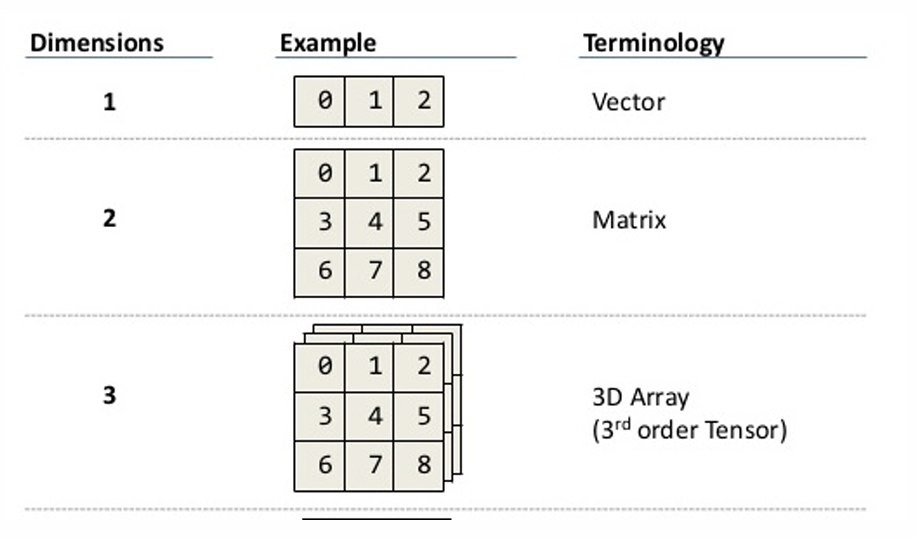
\includegraphics[width=0.75\linewidth]{Images/terminology-linalg.png}
    \caption{Linear Algebra Terminology}
\end{figure}


norm has to have certain properties!
L0 norm is not really a norm!.

infinity norm -> pick the maximum!

frobenius norm is just l2 norm of matrices

\end{document}
